\documentclass[a4paper,12pt]{article}
\usepackage{fancyhdr}
\usepackage[MeX]{polski}
\usepackage[utf8]{inputenc}
%\usepackage{amsmath,amsthm,amssymb}
\usepackage{graphicx}
%\usepackage[pdftex]{graphicx}


\pagestyle{fancy}
\lhead{Disaster manager}
\rhead{Dokument Wizji}

\author{Paweł Kimel, Tomasz Wasilczyk}
\title{Disaster manager}

\setlength{\headheight}{14.5pt}

\makeatletter
	\renewcommand\@seccntformat[1]{\csname the#1\endcsname.\quad}
	\renewcommand\numberline[1]{#1.\hskip0.7em}
	\renewcommand{\labelitemi}{-}
\makeatother

\renewcommand\maketitle
{
	\begin{titlepage}
	\begin{center}
	
	\textsc{Information Technology Infrastructure Library\\Service Delivery\\IT Service Continuity Management}\\[6cm]
	Paweł Kimel, Tomasz Wasilczyk\\[1cm]
	\textsc{\Large Disaster manager}\\[0.25cm]
	\textsc{\large Dokument Wizji}\\[8.675cm]
	
	\end{center}
	\end{titlepage}
}

\begin{document}

\maketitle

\setcounter{page}{2}

\tableofcontents

\break

%%%%%%%%%%%%%%%%%%%%%%%%%%%%%%%%%%%%%%%%%%%%%%%%%%%%%%%%%%%%%%%%%%%%%%%%%%%

\section{Słownik pojęć}

\begin{description}

	\item[Information Technology Infrastructure Library] (ITIL) -- zbiór zale-\\ceń i kodeks
	postępowania dla działów informatyki.

	\item[IT Service Continuity Management] (ITSCM) -- proces ITIL zarządzający ciągłością
	usług IT w przypadku zaistnienia sytuacji kryzysowych.

	\item[IT Service Availability Management] -- proces ITIL zarządzający dostępnością
	usług IT w trakcie codziennego użytkowania.

	\item[Procedura] -- określony przez użytkownika plan działania, złożony ze zdarzeń
	wykonywanych w określonej kolejności.

	\item[Zdarzenie] -- podstawowy składnik procedury, akcja wykonywana przez system ITSCM.

	\item[Czujnik] -- proces, lub urządzenie monitorujące stan usługi lub sprzętu,
	komunikujące się z systemem ITSCM.

\end{description}

%%%%%%%%%%%%%%%%%%%%%%%%%%%%%%%%%%%%%%%%%%%%%%%%%%%%%%%%%%%%%%%%%%%%%%%%%%%

\section{Wprowadzenie}

Aplikacja umożliwia zarządzanie bazą procedur awaryjnych (tworzenie, modyfikacja), wspomaga testowanie
i użycie ich w sytuacji kryzysowej. Ma także możliwość monitorowania, czy doszło do sytuacji kryzysowej,
co skraca czas wykrycia problemu i uruchomienia procedur.

Strona projektu (wraz z kodem źródłowym) znajduje się pod adresem: \textbf{disaster-manager.googlecode.com}.

%%%%%%%%%%%%%%%%%%%%%%%%%%%%%%%%%%%%%%%%%%%%%%%%%%%%%%%%%%%%%%%%%%%%%%%%%%%

\section{Ogólny opis produktu}

Aplikacja jest adresowana do średnich firm wykorzystujących w pracy systemy IT i posiadających
wyspecjalizowany dział IT. Realizuje zalecenia ITIL w dziedzinie IT Service Continuity Management,
czyli zarządzania usługami i ich ciągłością w sytuacjach kryzysowych.

\subsection{Możliwości}

Aplikacja umożliwia m.in. budowanie procedur awaryjnych. Składają się one z instrukcji warunkowych oraz zdarzeń, takich jak:

\begin{itemize}

	\item wyświetlenie komunikatu operatorowi,

	\item wysłanie wiadomości wskazanym osobom i wybranym kanałem (e-mail, SMS, komunikator internetowy),
	odbieranie informacji zwrotnej,

	\item wyłączanie usług, poinformowanie usługi o sytuacji awaryjnej,

	\item uruchomienie przywracania danych i usług,

	\item wykonanie innej procedury.

\end{itemize}

Wykonywane procedury są nadzorowane pod kątem przebiegu i odstępu czasowego pomiędzy
poszczególnymi zdarzeniami, co pozwala na wykonanie późniejszych analiz.

Przykładem innej funkcji realizowanej przez aplikację jest testowanie procedur, polegające
na wykonaniu ich z pominięciem pewnego podzbioru zdarzeń, ustalanego indywidualnie dla każdego testu.

Aplikacja monitoruje także stan czujników i -- w zależności od ustawień -- automatyczne
uruchamia określone procedury.

\subsection{Wymagania}

Aplikacja wymaga wdrożonego IT Service Availability Management nadzorującego pracę opisywanego systemu.
W przypadku uwzględnienia w procedurach zarządzania usługami, aplikacja musi mieć uprawnienia do ich obsługi.

Personel firmy powinien być przeszkolony w postępowaniu w sytuacji awaryjnej i we współpracy z systemem.
Operator aplikacji powinien być członkiem działu IT.

%%%%%%%%%%%%%%%%%%%%%%%%%%%%%%%%%%%%%%%%%%%%%%%%%%%%%%%%%%%%%%%%%%%%%%%%%%%

\section{Cechy produktu}

\begin{center}
	\begin{tabular}{|l|c|c|c|}
	
		\hline
	
		\textbf{cecha} & \textbf{status} & \textbf{wysiłek} & \textbf{priorytet} \\
	
		\hline
	
		aplikacja webowa & zatwierdzone & n/d & n/d \\
	
		\hline

		język: Java w technologii Servlet & zatwierdzone & n/d & n/d \\

		\hline

		obsługa kanału e-mail & zatwierdzone & mały & wysoki \\
		
		\hline

		obsługa kanału SMS & proponowane & średni & wysoki \\
		
		\hline

		obsługa kanału Jabber & zatwierdzone & średni & niski \\
		
		\hline

		czujniki programowe & zatwierdzone & wysoki & wysoki \\
		
		\hline

		czujniki sprzętowe & proponowane & wysoki & niski \\
		
		\hline

	
	\end{tabular}
\end{center}

%%%%%%%%%%%%%%%%%%%%%%%%%%%%%%%%%%%%%%%%%%%%%%%%%%%%%%%%%%%%%%%%%%%%%%%%%%%

\section{Podstawowe przypadki użycia}

\subsection{Dodanie procedury}

\begin{itemize}
	\item Użytkownik loguje się do systemu,

	\item wybiera opcję tworzenia nowej procedury,

	\item układa procedurę z dostępnych typów zdarzeń i uzupełnia związane z~nimi informacje,

	\item określa czasy wykonywania poszczególnych zdarzeń, oraz zdarzenia wykonywane w przypadku przekroczenia czasu,

	\item zatwierdza procedurę.
\end{itemize}

\subsection{Testowanie procedury}

\begin{itemize}
	\item Użytkownik loguje się do systemu,

	\item wybiera opcję testowania wybranej procedury,

	\item określa, które zdarzenia mają być wykonane,

	\item zatwierdza wykonanie tak ograniczonej procedury,

	\item raport z wykonania testu zostaje zapisany w bazie, użytkownik może go przejrzeć.
\end{itemize}

\subsection{Określenie automatycznej reakcji systemu na sygnały z czujników}

\begin{itemize}
	\item Użytkownik loguje się do systemu,

	\item wybiera opcję dodania nowej reakcji,

	\item określa monitorowany czujnik,

	\item określa przedziały wartości przy których nastąpi reakcja systemu i odpowiadające im procedury,

	\item zatwierdza wybór.
\end{itemize}

%%%%%%%%%%%%%%%%%%%%%%%%%%%%%%%%%%%%%%%%%%%%%%%%%%%%%%%%%%%%%%%%%%%%%%%%%%%

\section{Schemat bazy danych}

\begin{center}
	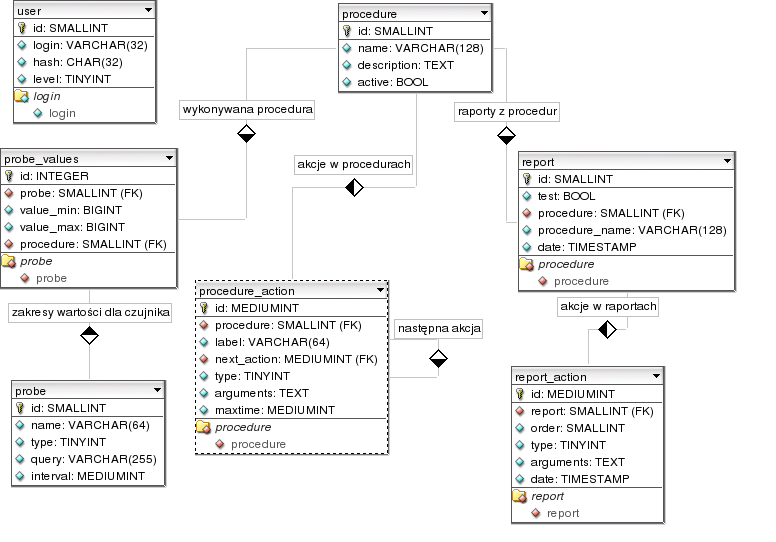
\includegraphics[width=135mm]{db-schema.png}
\end{center}

%%%%%%%%%%%%%%%%%%%%%%%%%%%%%%%%%%%%%%%%%%%%%%%%%%%%%%%%%%%%%%%%%%%%%%%%%%%

\section{Widoki}

\subsection{Edycja procedur}

\begin{center}
	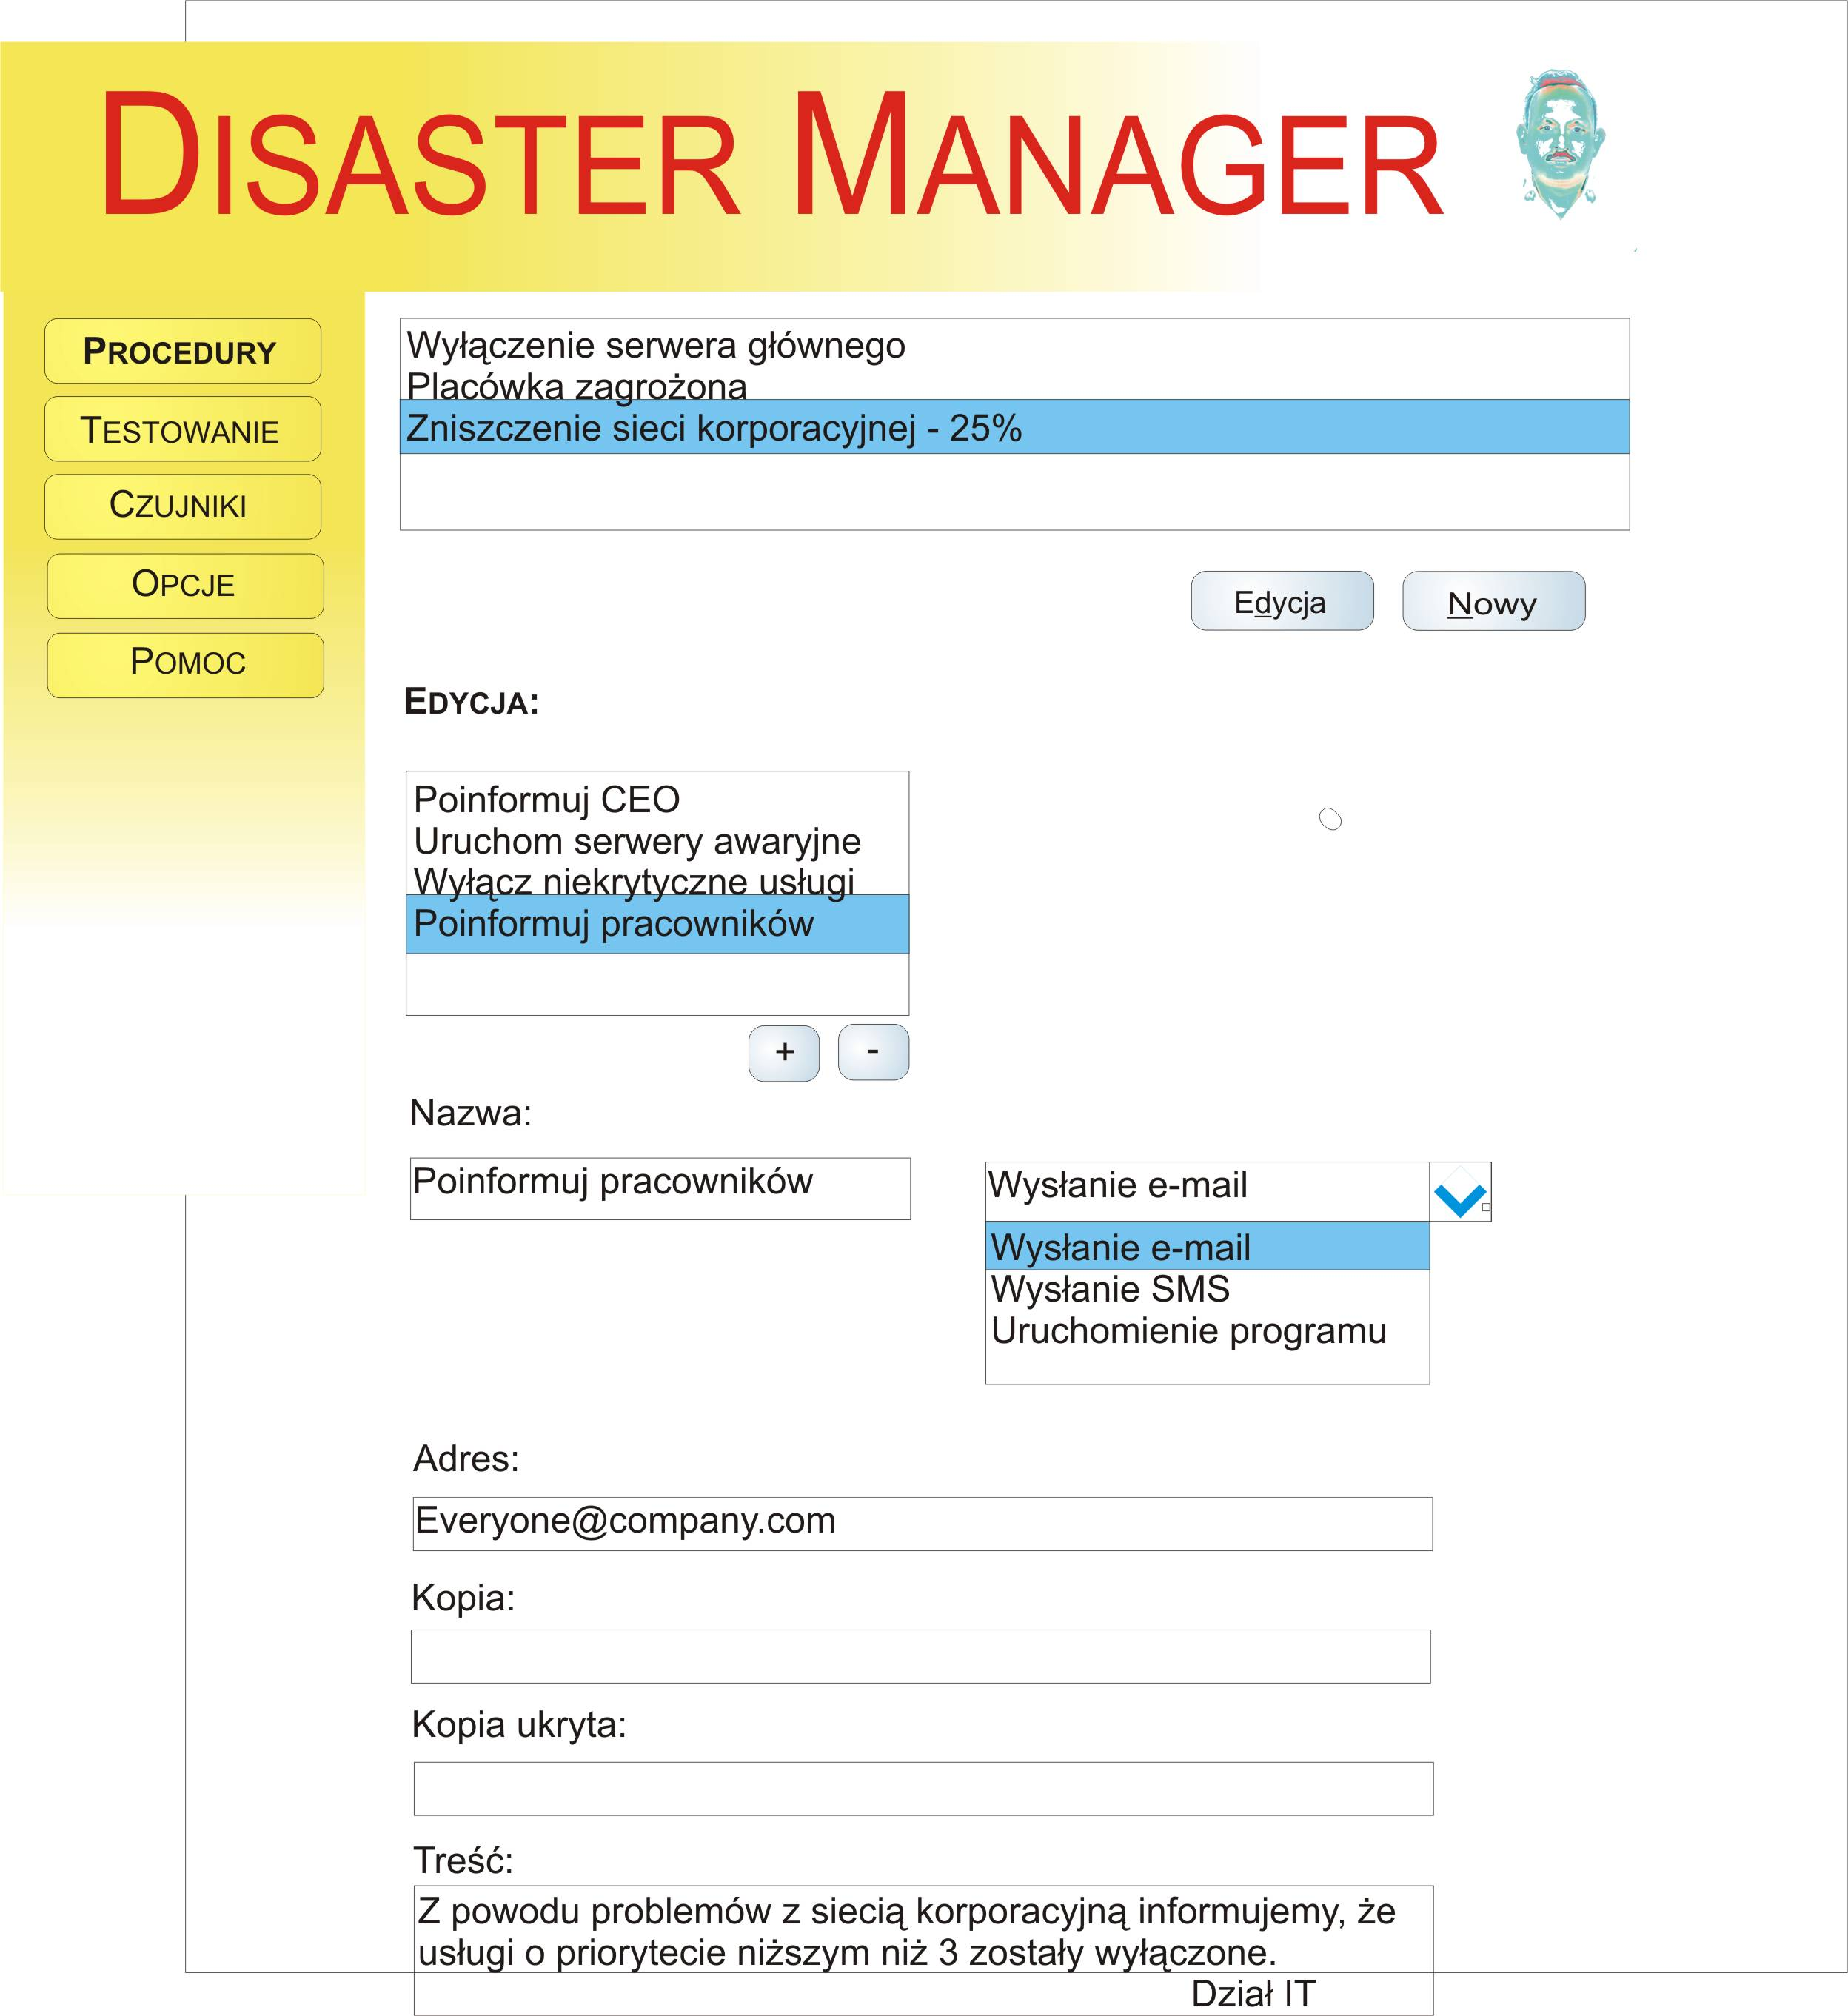
\includegraphics[width=135mm]{widoki/procedury.jpg}
\end{center}

%%%%%%%%%%%%%%%%%%%%%%%%%%%%%%%%%%%%%%%%%%%%%%%%%%%%%%%%%%%%%%%%%%%%%%%%%%%

\section{Terminarz}

\subsection{Iteracja pierwsza}

\begin{itemize}
	\item Przygotowanie frameworka servletu,
	\item opracowanie procedur obsługi zapytań (wybierania odpowiedniego kontrolera i akcji),
	\item implementacja klasy obsługi bazy danych,
	\item implementacja silnika szablonów odpowiedzi,
	\item kontroler obsługi stron błędów.
\end{itemize}


\subsection{Iteracja druga}

\begin{itemize}
	\item System logowania,
	\item panel zarządzania użytkownikami,
	\item panel dodawania i edycji procedur,
	\item moduł testowania procedur.
\end{itemize}


\subsection{Iteracja trzecia}

\begin{itemize}
	\item Obsługa kanałów komunikacji z użytkownikami,
	\item implementacja czujników programowych,
	\item projekt, budowa prototypu i oprogramowanie czujnika sprzętowego,
\end{itemize}

%%%%%%%%%%%%%%%%%%%%%%%%%%%%%%%%%%%%%%%%%%%%%%%%%%%%%%%%%%%%%%%%%%%%%%%%%%%

\end{document}